\documentclass[aspectratio=169, 10pt]{beamer}

\usepackage{bm} % bold math
\usepackage{fontspec}
\usepackage{minted}
\usepackage{pgf-pie}
\usepackage{tikz}
\usepackage{graphicx}
\newcommand\sbullet[1][.5]{\mathbin{\vcenter{\hbox{\scalebox{#1}{$\bullet$}}}}}

% Custom commands and environments
\makeatletter
\newcommand\version[1]{\renewcommand\@version{#1}}
\newcommand\@version{}
\def\insertversion{\@version}

\newcommand\course[1]{\renewcommand\@course{#1}}
\newcommand\@course{}
\def\insertcourse{\@course}

\newcommand\coursetitle[1]{\renewcommand\@coursetitle{#1}}
\newcommand\@coursetitle{}
\def\insertcoursetitle{\@coursetitle}

\newcommand\lecturenumber[1]{\renewcommand\@lecturenumber{#1}}
\newcommand\@lecturenumber{}
\def\insertlecturenumber{\@lecturenumber}
\makeatother

\newcommand{\slidetitle}[1]{{\xbseries \large \structure{#1}} \bigskip}
\newcommand{\term}[1]{{\color{blue} #1}}
\newcommand{\leftspace}{\hspace{1em}}
\newcommand{\inlinearrow}{
  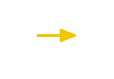
\begin{tikzpicture}[baseline]
    \node [anchor=base] (x) {};
    \draw [rawarrow] (x.mid west) -- ($(x.mid west) + (2em,0)$);
  \end{tikzpicture}
}

\newenvironment{slide}
{\begin{frame}[fragile,environment=slide]\vskip0pt plus 1filll}
{\vskip0pt plus 1filll\end{frame}}

% LaTeX

\setlength{\leftmargini}{1em}

% Common Information

\author{Talia Xu}
\course{COMPSCI 340}
\coursetitle{Operating Systems}
\date{2024 Semester 2}

% fontspec

\defaultfontfeatures{Ligatures=TeX}
% \setmainfont{Domine}
\setsansfont{Inter}[
  FontFace={ul}{n}{Font=*-Thin},
  FontFace={el}{n}{Font=*-ExtraLight},
  FontFace={l}{n}{Font=*-Light},
  FontFace={sb}{n}{Font=*-SemiBold},
  FontFace={eb}{n}{Font=*-ExtraBold},
  FontFace={xb}{n}{Font=*-Black},
]
\setmonofont[Contextuals=AlternateOff, Ligatures=TeXOff]{Iosevka}[
  FontFace={xb}{n}{Font=*-Heavy},
]

%% Font Weights

\DeclareRobustCommand{\ulseries}{\fontseries{ul}\selectfont}
\DeclareTextFontCommand{\textul}{\ulseries}
\DeclareRobustCommand{\elseries}{\fontseries{el}\selectfont}
\DeclareTextFontCommand{\textel}{\elseries}
\DeclareRobustCommand{\lseries}{\fontseries{l}\selectfont}
\DeclareTextFontCommand{\textl}{\lseries}
\DeclareRobustCommand{\sbseries}{\fontseries{sb}\selectfont}
\DeclareTextFontCommand{\textsb}{\sbseries}
\DeclareRobustCommand{\ebseries}{\fontseries{eb}\selectfont}
\DeclareTextFontCommand{\texteb}{\ebseries}
\DeclareRobustCommand{\xbseries}{\fontseries{xb}\selectfont}
\DeclareTextFontCommand{\textxb}{\xbseries}

% tikz

\usetikzlibrary{
  arrows,
  arrows.meta,
  automata,
  backgrounds,
  calc,
  decorations.pathreplacing,
  matrix,
  positioning,
  overlay-beamer-styles,
  shapes,
  shapes.multipart,
  tikzmark,
}

\tikzstyle{rawarrow} = [
  -{Latex[round]},
  line width=1pt,
  yellow,
  shorten >=3pt,
  shorten <=3pt,
  font=\small,
  text=black,
]

\tikzstyle{arrow} = [
  -{Latex[round]},
  line width=1pt,
  yellow,
  shorten >=3pt,
  shorten <=3pt,
  transform canvas={yshift=3pt},
  font=\small,
  text=black,
]

\newcommand{\tikzmarkcoord}[1]{([yshift=3pt]pic cs:#1)}

% minted

\setminted{style=eyolfson, fontsize=\small, escapeinside=||}
\setmintedinline{fontsize=\normalsize}

% hyperref

\hypersetup{colorlinks, urlcolor=blue}

% beamer
\setbeamersize{text margin left=16mm, text margin right=16mm}
\setbeamertemplate{itemize items}[circle]
\setbeamercolor{item}{fg=black}
\setbeamercolor{structure}{fg=darkblue}
\setbeamerfont{frametitle}{series=\bfseries, parent=structure}
\setbeamertemplate{navigation symbols}{}
\setbeamertemplate{headline}{}
\setbeamertemplate{footline}{
  \begin{tikzpicture}[
    remember picture,
    overlay,
    shift={(current page.south west)},
  ]
    \path [fill=gray] (144mm, 0) -- (160mm, 16mm) -- (160mm, 0);
    \node [inner sep=3.5mm, outer sep=0, text=black, anchor=base east,
           align=right, yshift=3.5mm]
          at (current page.south east) {\ttfamily \small \insertframenumber{}};
  \end{tikzpicture}
}
\setbeamertemplate{title page}{
  \begin{tikzpicture}[
    remember picture,
    overlay,
    shift={(current page.south west)},
    background rectangle/.style={fill=darkblue},
    show background rectangle,
  ]
    \node [anchor=center, align=center, text=white, text width=40mm, scale=3.2]
          at (\paperwidth / 2, \paperheight * 2 / 3)
          {\xbseries \inserttitle{}};
    \node [anchor=base west, align=left, inner sep=0, text=white, yshift=2.5mm]
          at (16mm, \paperheight / 3)
          {\insertdate{} \insertcourse{}: \insertcoursetitle{}};
    \node [anchor=base west, align=left, inner sep=0, text=white, yshift=-2.5mm]
          at (16mm, \paperheight / 3)
          {\insertauthor};
    \node [anchor=base east, align=right, inner sep=0, text=white, yshift=2.5mm]
          at (144mm, \paperheight / 3)
          {Lecture \insertlecturenumber{}};
    \node [anchor=base east, align=right, inner sep=0, text=white,
           yshift=-2.5mm]
          at (144mm, \paperheight / 3)
          {\ttfamily \insertversion{}};
    \node [align=center, anchor=south, inner sep=0, text=white, yshift=3.5mm]
          (license) at (\paperwidth / 2, 0)
          {\fontsize{7pt}{7pt}\selectfont This  work is licensed under a
           \href{http://creativecommons.org/licenses/by-sa/4.0/}
                {\color{lightblue} Creative Commons Attribution-ShareAlike 4.0
                 International License}};
  \end{tikzpicture}
}

% xcolor

%% Primary Colour

\definecolor{pantone655}{RGB}{0, 42, 92} % #002a5c
\colorlet{darkblue}{pantone655}

%% Secondary Colours

\definecolor{pantone633}{RGB}{0, 139, 176} % #008bb0
\colorlet{blue}{pantone633}

\definecolor{pantonewarmred}{RGB}{220, 70, 51} % #dc4633
\colorlet{red}{pantonewarmred}

\definecolor{pantone3285}{RGB}{0, 161, 137} % #00a189
\colorlet{cyan}{pantone3285}

\definecolor{pantone7722}{RGB}{13, 83, 77} % #0d534d
\colorlet{darkcyan}{pantone7722}

\definecolor{pantone376}{RGB}{141, 191, 46} % #8dbf2e
\colorlet{green}{pantone376}

\definecolor{pantone2613}{RGB}{109, 36, 122} % #6d247a
\colorlet{violet}{pantone2613}

\definecolor{pantone2985}{RGB}{111, 199, 234} % #6fc7ea
\colorlet{lightblue}{pantone2985}

\definecolor{pantone227}{RGB}{171, 19, 104} % #ab1368
\colorlet{magenta}{pantone227}

\definecolor{pantone7406}{RGB}{241, 197, 0} % #f1c500
\colorlet{yellow}{pantone7406}

%% Neutrals

\definecolor{pantonecoolgray2}{RGB}{208, 209, 201} % #d0d1c9
\colorlet{gray}{pantonecoolgray2}


\lecturenumber{17}
\title{Threads\\Implementation}
\version{2.0.0}

\begin{document}

  \begin{frame}[plain, noframenumbering]
    \titlepage
  \end{frame}

  \begin{slide}

    \slidetitle{Multithreading Models}

    Where do we implement threads?

    \leftspace{}We can either do user or kernel threads
    \medskip

    User threads are completely in user-space

    \leftspace{}Kernel doesn't treat your threaded process any differently
    \medskip

    Kernel threads are implemented in kernel-space

    \leftspace{}Kernel manages everything for you, and can treat threads specially

  \end{slide}

  \begin{slide}
    \slidetitle{Thread Support Requires a Thread Table}

    Similar to the process table we saw previously
    
    \leftspace{}It could be in user-space or kernel-space (depending)
    \medskip

    For user threads, there also needs to be a run-time system to determine
    scheduling
    \medskip

    In both models each process can contain multiple threads

  \end{slide}

  \begin{slide}

    \slidetitle{We Could Avoid System Calls, or Let a Thread Block Everything}

    For pure user-level threads (again, no kernel support):

    \begin{itemize}
      \item Very fast to create and destroy, no system call, no context switches
      \item One thread blocks, it blocks the entire process (kernel can't distinguish)
    \end{itemize}
    \medskip

    For kernel-level threads:

    \begin{itemize}
      \item Slower, creation involves system calls
      \item If one thread blocks, the kernel can schedule another one
    \end{itemize}

  \end{slide}

  \begin{slide}

    \slidetitle{All Threading Libraries You Use Run in User-mode}

    The thread library maps user threads to kernel threads
    \medskip

    Many-to-one: threads completely implemented in user-space

    \leftspace{}the kernel only sees one process
    \medskip

    One-to-one: one user thread maps directly to one kernel thread

    \leftspace{}the kernel handles everything
    \medskip

    Many-to-many: many user-level threads map to many kernel level threads

  \end{slide}

  \begin{slide}

    \slidetitle{Many-to-one is Pure User-space Implementation}

    It's fast (as outlined before) and portable

    \leftspace{}It doesn't depend on the system, it's just a library
    \medskip

    Drawbacks are that one thread blocking causes all threads to block

    \leftspace{}Also, we cannot execute threads in parallel

    \leftspace{}\leftspace{}The kernel will only schedule a process to run

  \end{slide}

  \begin{slide}

    \slidetitle{One-to-one Just Uses the Kernel Thread Implementation}

    There's just a thin wrapper around the system calls to make it easier to use
    \medskip

    Exploits the full parallelism of your machine

    \leftspace{}The kernel can schedule multiple threads simultaneously
    \medskip

    We do however need to use a slower system call interface,

    \leftspace{}and we lose some control
    \bigskip

    Typically, this is the actual implementation used, we'll assume this for
    Linux

  \end{slide}

  \begin{slide}

    \slidetitle{Many-to-many is a Hybrid Approach}

    The idea is that there are more user-level threads than kernel-level threads

    \leftspace{}Cap the number of kernel-level threads to the number we could
    run in parallel
    \medskip

    We can get the most out of multiple CPUs and reduce the number of system
    calls
    \medskip

    However, this leads to a complicated thread library (Java Virtual Threads)

    \leftspace{}Depending on your mapping luck, you may block other threads

  \end{slide}

  \begin{slide}

    \slidetitle{Threads Complicate the Kernel}

    How should \texttt{fork} work with a process with multiple threads?

    \leftspace{}Copy all threads to the new process, in whatever state they're
    in?

    \leftspace{}\leftspace{}How would this get out of hand?
    \medskip

    Linux only copies the thread that called \texttt{fork} into a new process

    \leftspace{}If it hits \texttt{pthread\_exit} it'll always exit with
                  status 0

    \leftspace{}\leftspace{}(at least as far as I can tell)
    \medskip

    There's \texttt{pthread\_atfork} (not covered in this course) to control
    what happens

  \end{slide}

  \begin{slide}

    \slidetitle{Signals are Sent to a Process}

    Which thread should receive a signal? all of them?
    \medskip

    Linux will just pick one random thread to handle the signal

    \leftspace{}Makes concurrency hard, any thread could be interrupted

  \end{slide}

  \begin{slide}

    \slidetitle{Instead of Many-to-many, You Can Use a Thread Pool}

    The goal of many-to-many thread mapping is to avoid creation costs
    \medskip

    A thread pool creates a certain number of threads and a queue of tasks

    \leftspace{}(maybe as many threads as CPUs in the system)
    \medskip

    As requests come in, wake them up and give them work to do
    \medskip

    Reuse them, when there's no work, put them to sleep

  \end{slide}

  \begin{slide}

    \slidetitle{You'll Implement Many-to-one}

    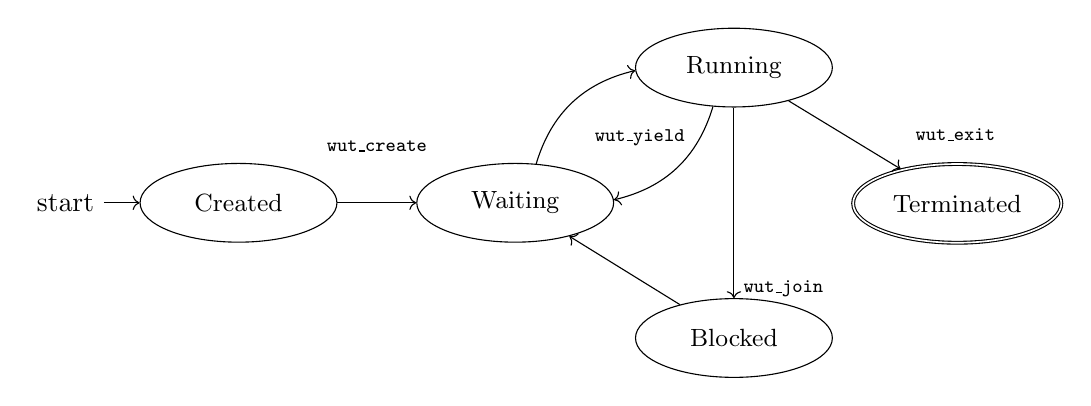
\begin{tikzpicture}[
      every state/.style={ellipse, minimum width=2.5cm, minimum height=1cm, font=\small},
    ]
      \node [state, initial] (created) {Created};
      \node [state, right=of created] (waiting) {Waiting};
      \node [state, above right=of waiting] (running) {Running};
      \node [state, below right=of waiting] (blocked) {Blocked};
      \node [state, accepting, below right=of running] (terminated) {Terminated};
      \path [->] (created) edge (waiting) node [above, xshift=5em, yshift=1.5em] {\scriptsize \ttfamily wut\_create}
                 (waiting) edge [bend left] (running) node [below, xshift=4.5em, yshift=3em] {\scriptsize \ttfamily wut\_yield}
                 (running) edge [bend left] (waiting)
                 (running) edge (blocked) node [right, yshift=-8em] {\scriptsize \ttfamily wut\_join}
                 (blocked) edge (waiting)
                 (running) edge (terminated) node [above, xshift=8em, yshift=-3em] {\scriptsize \ttfamily wut\_exit};
    \end{tikzpicture}

  \end{slide}

  \begin{slide}

    \slidetitle{Your Scheduler Can Just Be Round Robin}

    Create a queue (list), run the thread at the front, when it yields at it to the back
    \medskip

    You'll have to do the context switch (remember, you'll have to save the registers)
    \medskip

    These are cooperative threads, so they have to be nice (next is preemptive threads)

  \end{slide}

  \begin{slide}

    \slidetitle{Our Next Complication}

    Let's create a program that spawns 8 threads

    \leftspace{}Each thread increments the same variable 10,000 times
    \medskip

    What should the final value of the variable be?

    \leftspace{}The initial value of the variable is 0
    \medskip

    Run \texttt{lectures/17-threads-implementation/pthread-datarace}

    \leftspace{}Can you fix it?

  \end{slide}

  \begin{slide}

    \slidetitle{Both Processes and (Kernel) Threads Enable Parallelization}

    \begin{itemize}
      \item Each process can have multiple (kernel) threads
      \item Most implementations use one-to-one user-to-kernel thread mapping
      \item The operating system has to manage what happens during a fork, or signals
      \item We now have synchronization issues
    \end{itemize}

  \end{slide}

\end{document}
